\section{模型可解释性与温度作用分析}

\subsection{分析目标}

在药物研发与工艺设计中，高精度的机器学习模型若缺乏透明的决策逻辑，将难以赢得药物化学家的信任，更无法为分子修饰或工艺改进提供指导。本章聚焦两项核心机理问题：深入解析 ExtraTrees--TabPFN 模型的特征归因与 TabPFN 的局部校正路径，并系统探究温度与溶解度的物理因果关联，检验模型温度响应的真实性。

\subsection{SOLAR-H 结构贡献}

SOLAR-H 模型在数学架构上天然具备白盒透明度。根据式\eqref{eq:v2-solar}，模型输出严格由两部分线性叠加而成：
\begin{equation}
\widehat y_i = \underbrace{\widehat b(z_c)}_{\text{结构常数项}} + \underbrace{\gamma \cdot \tau_i \cdot \left( u_c^\top \widehat\beta \right)}_{\text{结构调制的温度响应项}}.
\end{equation}
对于任意固定的药物--溶剂组合 $c$，模型对温度的响应导数恒定为 $\frac{\partial \widehat y}{\partial T} = \frac{\gamma u_c^\top \widehat\beta}{s_T}$。在全量开发集部署配置中，由于内层嵌套验证自动选取了高阻尼增益 $\gamma = 0$，模型自适应退化为结构基线预测，有效杜绝了因温度噪声在未见母体上的外推漂移。当在训练折选用非零增益时，参数 $\widehat\beta$ 显式反映了分子量差异、极性失配对吸热溶解斜率的调节方向。

\subsection{特征归因}\label{sec:deployment-explanations}

对于非线性的 ExtraTrees--TabPFN 工业部署模型，本研究结合博弈论 Shapley 值与局部分支贡献展开双重归因分析。

\subsubsection{TreeSHAP 全局特征组归因分析}
对于 ExtraTrees 树分支，采用基于树路径依赖的 TreeSHAP 算法\cite{treeshap2020}。在 128 个开发母体中均衡抽取覆盖全量化学空间的 227 条解释样本。TreeSHAP 算法在浮点精度级别满足局部准确性公理（重构预测偏差低于 $1.3\times10^{-13}$），基线参考期望值（背景预测值）为 $-1.1632$。

将模型保留的 665 个高维特征按照化学物理属性归集为四大功能组：药物描述符、溶剂描述符、温度特征以及显式分子间交互特征。各组的有符号归因绝对值在 128 个母体维度等权平均后的结果如图~\ref{fig:deployment-explanations}A 所示。

\begin{figure}[htbp]
\centering
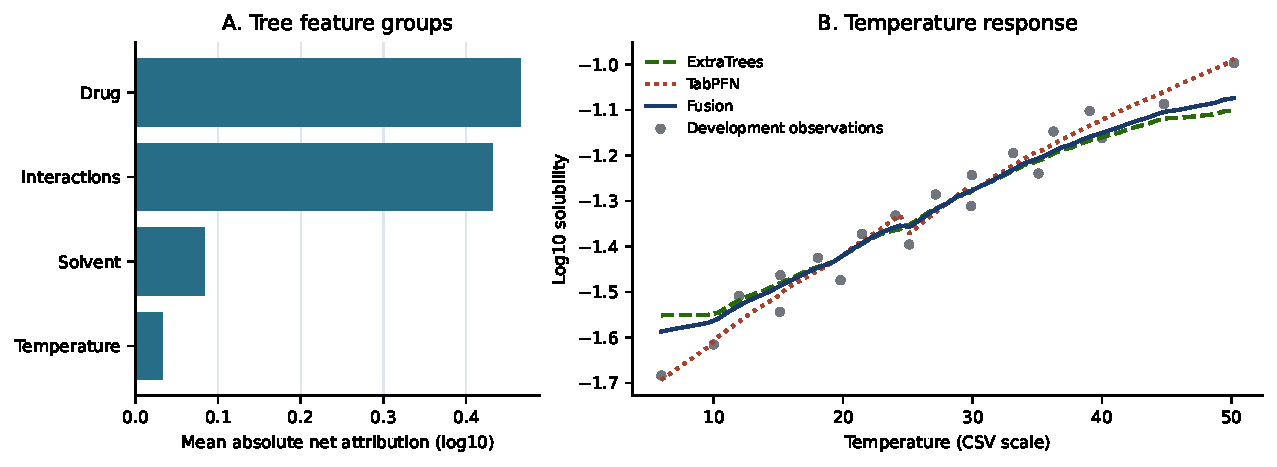
\includegraphics[width=\linewidth]{deployment_explanations.pdf}
\caption{部署模型的特征归因与温度动态响应分析。\textbf{A} 四大功能特征组的母体等权绝对净归因对比；\textbf{B} 洛伐他汀--乙酸丁酯组合在观测温区内的预测曲线（散点为真实测量点，实线为融合预测，虚线为各单分支响应）。}
\label{fig:deployment-explanations}
\end{figure}

归因结果具有明确的化学含义。药物描述符（平均绝对归因 0.466）与显式交互特征（0.432）的归因值最高。这与溶液物理化学一致：药物分子结构庞大复杂（分子量通常在 200--800 之间），其固态晶格能与固相内聚强度是溶解需要克服的晶格能项；而溶质与溶剂之间的显式交互（极性匹配与氢键配对）直接决定了溶剂化放热能否克服晶格能。相比之下，溶剂描述符（0.084）与温度特征（0.033）起精细微调作用。由于溶剂库相对有限（49 种常见工业溶剂）且结构较为规整，其单独贡献相对集中，更多作为条件扰动在宏观结构基线上进行局部调节。

\subsubsection{TabPFN 的局部分支动态校准机理}
为探究 TabPFN 如何与 ExtraTrees 协同工作，表~\ref{tab:deployment-examples}选取了部署模型中 TabPFN 修正量 $\Delta_{\mathrm{PFN}} = 0.25 (f_{\mathrm{PFN}} - f_{\mathrm{ET}})$ 呈现极大与极小极端调节的两条真实案例。

\begin{table}[htbp]
\centering\small
\setlength{\tabcolsep}{4pt}
\caption{部署模型中 TabPFN 对 ExtraTrees 分支进行双向微调校准的典型案例分析（两例均以丙酮为溶剂）。}
\label{tab:deployment-examples}
\begin{tabular}{lrrrrrr}
\toprule
候选药物（数据索引） & 温度 ($^\circ\text{C}$) & 实测值 & ExtraTrees & TabPFN & 融合预测 & 修正量 $\Delta_{\mathrm{PFN}}$ \\
\midrule
赤藓糖醇（样本行 23） & 13.2 & $-2.692$ & $-2.495$ & $-2.716$ & $-2.551$ & $-0.055$（下调） \\
对羟基苯甘氨酸 Dane 盐（样本行 3） & 70.2 & $-1.843$ & $-1.927$ & $-1.847$ & $-1.907$ & $+0.020$（上调） \\
\bottomrule
\end{tabular}
\end{table}

两项案例生动展现了异质集成的自适应校正机制。在赤藓糖醇案例中，ExtraTrees 受到常温多羟基化合物统计均值的牵引，对数预测为 $-2.495$（显著高估实测值 $-2.692$）。TabPFN 基于连续注意力空间识别出其高极性小分子在低极性溶剂中的不溶性特征，给出更低的 $-2.716$ 预测，驱动融合模型向下校正至 $-2.551$，大幅缩减了绝对误差。在 Dane 盐案例中，ExtraTrees 预测偏保守（$-1.927$），而 TabPFN 准确捕捉到 $70.2^\circ\text{C}$ 高温下的热力学促溶效应，给出 $-1.847$ 预测，驱动融合模型向上微调至 $-1.907$，逼近实测值 $-1.843$。上述对比确证了 TabPFN 依托其丰富的先验流形表征，在不同化学空间动态实施方向完全不同的有效纠偏。

\subsection{动态温度响应}

为检验模型在连续温度变化下的物理合理性，固定洛伐他汀--乙酸丁酯体系（该体系在开发集中包含 20 个密集的温度实测点，温区跨度为 $[5.95^\circ\text{C}, 50.2^\circ\text{C}]$），对输入温度进行等距致密扫描（图~\ref{fig:deployment-explanations}B）。

扫描曲线清晰地表明：ExtraTrees 表现出阶梯状分段非线性，反映了轴切分树模型的典型离散特性；而融合模型展现出平滑、单调向上的连续响应曲线，对数溶解度预测值从 $5.95^\circ\text{C}$ 下的 $-1.587$ 稳步递增至 $50.2^\circ\text{C}$ 下的 $-1.074$；预测曲线紧密穿过真实实验观测散点簇的中枢，高度符合大多数固液溶质吸热溶解的宏观物理热力学规律，证实模型学到了物理一致的温变行为。